%% Los cap'itulos inician con \chapter{T'itulo}, estos aparecen numerados y
%% se incluyen en el 'indice general.
%%
%% Recuerda que aqu'i ya puedes escribir acentos como: 'a, 'e, 'i, etc.
%% La letra n con tilde es: 'n.

\chapter{Marco Teórico}
\section{Descripción del Problema}

El término cliqué proviene de la palabra inglesa y francesa clique, que define a un grupo de personas que comparten intereses en común. En esta analogía, las personas serían los vértices; las relaciones de interés, las aristas; y el hecho de que todas compartan un mismo interés, el grafo completo, es decir, el clique en si.\\\\
Dado un grafo no dirigido cualquiera G= (V,E), en el cual V={1,2,...,n} es el conjunto de  los  vértices  del  grafo  y  E  es  el  conjunto  de  aristas.  Un  clique  es  un  conjunto  C  de  vértices  donde todo par de vértices de C esta conectado con una arista en G, es decir C es un subgrafo completo.

\section{Propuesta de Soluci'on}
Para poder dar soluci´on a este problema NP se propone utilizar un Algoritmo Recursivo, el cual no es el algoritmo más optimo para un grafo muy grande, sin embargo es desarrollado y propuesto por nosostros.

\chapter{Síntesis de lectura}

\section{Explicación}
El problema del máximo clique, donde debemos de encontrar el clique con la mayor cantidad de vértices dentro de un grafo dado
Tiene varias aplicaciones en diversos campos como la búsqueda comunitaria en: \\
\textbf{Redes y redes sociales}: Se busca conectar a las personas que están familiarizadas entre si como bordes y candidatos (cliques) para servir a otras comunidades, esto para crear una herramienta eficiente de análisis entre organizaciones y distintas redes en el estudio de estructuras mesoscópicas.
\\
\textbf{Formación de equipos en redes expertas:} Se captura la compatibilidad entre expertos así como sus capacidades individuales para formar equipos donde k-cliques cubre perfectamente un conjunto de capacidades donde k son el número de expertos.
\\
\textbf{Genética y bioinformática:} Donde los grupos de expresión genética (CEG) se modelan como cliques para encontrar grandes equipos en la genética de redes.
\\
\textbf{Detección de anomalías en redes complejas:} son usados para encontrar señales de eventos raros, como el reclutamiento de terrorista o el correo no deseado en la web.\\

En este articulo se busca un algoritmo aleatorio para el problema del máximo clique mediante diferentes enfoques como lo son en búsqueda de un vértice tras otro, enfoque RMC, clique máximo aleatorio, búsqueda binaria, etc. Donde el objetivo es encontrar una probabilidad de solución del problema \begin{math}
≥1-n^{-c}
\end{math} donde se determina el clique máximo mediante la búsqueda de iterativa de un clique-k en S a partir de  \begin{math} k= wc +1 \end{math} hasta que S se convierte en vacío mientras pasan las iteraciones. Sin embargo, debido a la dureza del problema todos estos algoritmos fallan cuando se enfrentan a gráficos masivos (debido al aumento de tecnologías web e internet), se han propuestos diversas soluciones con una buena tasa de probabilidad sobre el clique máximo.

Actualmente todos estos algoritmos tienen una deficiencia importante, ya que dependen del orden inicial del vértice. Por eso trabajaremos con un nuevo enfoque donde:
\\
\textbf{Primero:} Debido a la dureza del problema, se proponen soluciones al problema.
\\
\textbf{Segundo:} En lugar de usar un esquema de ramificación y unión, es decir, ramificar desde cada vértice para enumerar todos los cliques y poder ramificar, se propondrá un esquema de búsqueda binaria con topes en cada iteración hasta que ya no queden más iteraciones.
\\
\textbf{Tercero:} Que cada iteración de la búsqueda binaria se trabaje como un problema de k-cliques en S con una probabilidad de garantía \begin{math} ≥1-n^(-c) \end{math} donde para cada semilla en S introducimos una semilla sc y tci para reducir de forma iterativa los subgrafos generados. 
\\
\textbf{Cuarto:} Proponemos un nuevo algoritmo iterativo de fuerza bruta para determinar el clique máximo después de una búsqueda binaria desde \begin{math} k = wc + 1  \end{math} . 
\\
\textbf{Quinto:} Hacemos los estudios experimentales para mostrar la solidez y eficiencia de nuestro algoritmo y enfoque.
\\

\section{Definición del problema}

Modelaremos una red social como un gráfico no dirigido \begin{math} G =(V,E) \end{math} 
sin auto bucles o bordes múltiples, donde V y E denotan los conjuntos de vértices y bordes de G, donde n y m denotaran el número de vértices y aristas de G, es decir, \begin{math}
n = |V| y m = |E|
\end{math},donde se da por hecho que G esta conectado, de lo contrario, el algoritmo se puede aplicar a cada componente conectado en el grafo.
\\
Un grafo G es un clique si hay bordes entre 2 vértices de G. También llamamos a un conjunto de vértices CCV una camarilla si el subgrafo inducida por C es una camarilla. C es una camarilla máxima si no existe un superconjunto adecuado de C que también sea una camarilla y C es una camarilla máxima si no existe una camarilla C como tal \begin{math} | C '| > | C | \end{math}. El número de vértices en una camarilla máxima en el gráfico G = (V, E) se denota como w (G) o w (V). Por simplicidad, en la siguiente discusión, usamos \begin{math} ~ w (G) o ~ w (V)\end{math} para denotar el límite superior de la camarilla máxima de G = (V, E) y usamos w (G) o w (V) para representar el límite inferior de la camarilla máxima de G, respectivamente.
\\
\section{Trabajos relacionados}
\\
El clique se estudio por primera vez para modelar grupos de individuos que se conocen entre si y fue modelado por Cook y Karp utilizando la teoría de la completitud NP y los resultados de intratabilidad relacionados para proporcionar una explicación matemática de la dificultad del problema. Tarjan y Trojanowski dieron con el peor de los casos, en 1990 Feige demuestra que es imposible de aproximar el problema con precisión y eficacia hasta que se propone un algoritmo de tiempo polinómico O ((log logn)2) siempre que el gráfico tenga una camarilla de tamaño O \begin{math}n * log(nb)\end{math} para cualquier constante b. Pero todos estos trabajos son trabajados como grafos pequeños, pocos han aplicado para grafos realmente grandes utilizando métodos como listas de adyacencias, búsquedas binarias. La diferencia con este algoritmo es que ahora buscan limites superiores e inferiores para mejorar las soluciones por aproximación usando una búsqueda local dinámica y el uso de la diversificación, aplicado también en búsqueda tabú y redes neuronales.
\\
\textbf{Algoritmos anteriores}
Dejan que el clique máximo encontrado, denotada como Cm, como un límite inferior de w(G). Dejamos que C denote el clique actual, y P =(C) denote el conjunto candidato del cual se seleccionará un vértice para que C crezca a continuación. En otras palabras, poda ramas que no pueden generar cliques más grandes que Cm.
\\
\begin{figure}[h!]
\centering
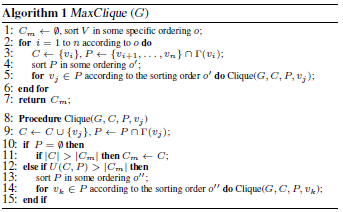
\includegraphics[scale=1.5]{img/imagen1.png}
\caption{Algoritmo 1}
\label{Comandos}
\end{figure}
\\
\begin{itemize}
    \item Línea 1: Lista en un orden.
    \item Línea 2: recorre hasta.
    \item Línea 3: Inicializa.
    \item Línea 4: Ordena en algún orden.
    \item Línea 5: Quita las ramas infructuosas.
    \item Línea 6: termina el proceso.
    \item Línea 7: regresa Cm.
    \item Línea 8: Procede con el clique.
    \item Línea 9: Actualiza y regresa un clique.
    \item Línea 10 y 11: Si encuentra un clique, entonces se actualiza.
    \item Línea 12 a 14: De lo contrario no encuentra un clique más grande.
\end{itemize}
\\
Los algoritmos anteriores funcionan bien en muchas redes. Sin embargo, se enfrentan a desafíos cada vez mayores cuando se trata de redes de rápido crecimiento en la vida real. En el fondo de las soluciones existentes y los gráficos masivos del mundo real, observamos tres razones principales que perjudican enormemente la eficiencia y la solidez de los algoritmos existentes.
\\
\textbf{Primero:} El conjunto candidato es muy grande y no tiene un límite fijo, va cambiando.
\\
\textbf{Segundo:} En la practica los vértices de alto grado siempre tienen una gran cantidad de bordes que se conectan con vértices de bajo grado
\\
\textbf{Tercero:} No se utiliza el límite superior de w(G) en los algoritmos existentes. Pierde tiempo para buscar ramas restantes
\\
\textbf{Visión general del enfoque}
Se diseña un nuevo algoritmo aleatorio basado en la búsqueda binaria, para mejorar significativamente la robustez y la eficiencia del algoritmo. El algoritmo mantiene un limite inferior y superior de w(G) e intenta encontrar el clique máximo con algunas diferencias. 
En nuestra búsqueda binaria, en lugar de encontrar una camarilla wt en una iteración directamente, encontramos un conjunto de subgrafos donde pueden existir camarillas wt. El conjunto se denota de la siguiente manera.
\\
\begin{figure}[h!]
\centering
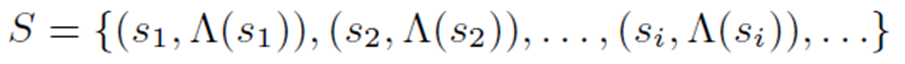
\includegraphics[scale=1]{img/imagen2.png}
\label{Comandos}
\end{figure}
\\
Donde (si, \begin{math}\Delta\end{math} (si)) es un subgrafo que consiste en una camarilla si y un conjunto candidato  \begin{math}\Delta\end{math} (si) desde el cual el clique puede crecer. Para simplificar, utilizamos el término "semilla" para representar tanto la camarilla si como el subgrafo (si,  \begin{math}\Delta\end{math} (si)). Además, cada (si,  \begin{math}\Delta\end{math} (si)) está asociado con una menor obligado wi y un límite superior ~wi de w (si U  \begin{math}\Delta\end{math} (si)), y todos estos límites se pueden combinar para actualizer wc y ~wc, st, wc = maxi{wi} y ~wc = maxi{~wi}, que a cambio poda las semillas sin fruto.
Determinamos los límites inferior y superior para la próxima iteración. Sea wc y ~wc los límites actuales, y sea wp y ~wp los límites anteriores. Hay 4 casos como se ilustra en la Fig. 2 basados en wc y ~wc.
1) El caso óptimo: si S ≠ 0 y wc ≥ wt, que es equivalente a wc = ~ wc, se ha encontrado el clique máximo y el algoritmo termina.
2) Si S ≠ 0 y wc < ~wt, entonces G no contiene cliques, disminuya ~ wc como wt - 1).
3) Si S ≠ 0 wc  ≠ wp o ~ wc ≠ ~ wp, más iteraciones pueden mejorar los límites.
4) Si S ≠ 0, wc = wp y ~wc =~wp, otras iteraciones introducen mejoras marginales, finaliza la búsqueda binaria y aplica un algoritmo de búsqueda de fuerza bruta.
\\
\begin{figure}[h!]
\centering
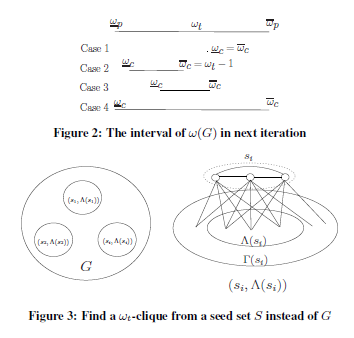
\includegraphics[scale=1.5]{img/imagen3.png}
\caption{Intérvalo w(G)}
\label{Comandos}
\end{figure}
\\
\subsection{Pasos a seguir}
\begin{enumerate}
    \item Muestreo de los bordes de G con probabilidad.
    \item Generar semillas en triángulos abiertos para que tenga probabilidad de clique.
    \item Encuentra el clique máximo en G.
\end{enumerate}

\subsection{Reducción por k-núcleo}
Agrandar s y reducir \begin{math}\Delta\end{math} (s) de la siguiente manera.

\begin{figure}[h!]
\centering
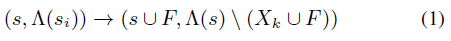
\includegraphics[scale=1]{img/imagen7.png}
\label{Comandos}
\end{figure}

Aquí Xk es un subconjunto de \begin{math}\Delta\end{math} (s) que no puede existir en a (k - |s|- 1) -núcleo en \begin{math}\Delta\end{math} (s) para una k dada, y F es un conjunto de vértices que tienen el potencial de existir en una camarilla máxima de \begin{math}\Delta\end{math} (s) donde F \begin{math}\Delta\end{math} (s) n Xk. Hay dos condiciones para que se seleccione F.
\begin{enumerate}
    \item Cada vértice en F está conectado a cada vértice en si, lo cual está garantizado por la definición de \begin{math}\Delta\end{math} (si).
    \item Cada vértice en F está conectado a cualquier otro vértice en \begin{math}\Delta\end{math} (s) n Xk. En otras palabras, F es una clique a tener en cuenta.
\end{enumerate}
\\
\begin{figure}[h!]
\centering
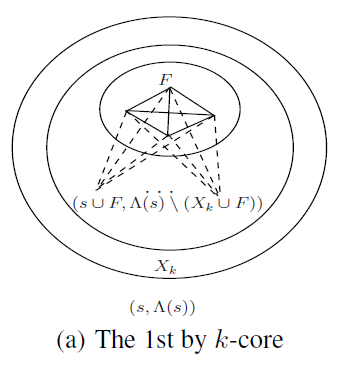
\includegraphics[scale=.5]{img/imagen4.png}
\caption{Reducción por k-núcleo}
\label{Comandos}
\end{figure}
\\
\subsection{Reducción por k-truss, coloración y conjunto independiente}
Basado en el anterior, pero con un nuevo enfoque donde:
\\
\begin{figure}[h!]
\centering
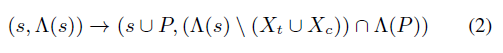
\includegraphics[scale=1]{img/imagen5.png}
\label{Comandos}
\end{figure}
\\
Mediante el truss k, identificamos Xt, que es un subconjunto de \begin{math}\Delta\end{math} (s) que no puede existir, coloreamos, identificamos Xc \begin{math}\Delta\end{math} (s) n Xt que contiene vértices cuyos vecinos se pueden colorear con menos de wt - |s| -1 colores, por lo tanto, el clique no contiene vertices en Xt.
\\
\begin{figure}[h!]
\centering
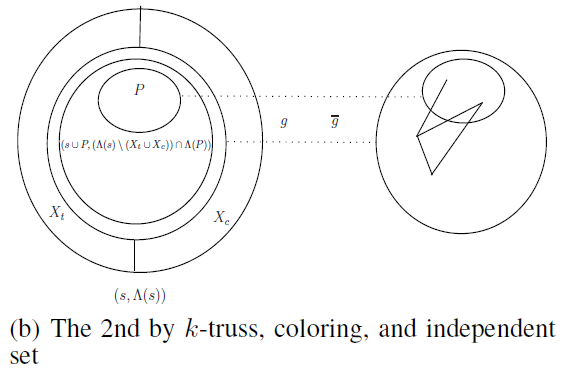
\includegraphics[scale=1.1]{img/imagen6.png}
\caption{Reducción por k-truss}
\label{Comandos}
\end{figure}
\\
El segundo círculo más grande a la izquierda representa un subgrafo g de (s, \begin{math}\Delta\end{math} (s)) al excluir los vértices en (Xt U Xc). Reducimos aún más g usando un conjunto independiente. Sea g la gráfica complementaria de g (el círculo más grande a la derecha). Con la ayuda de un conjunto independiente encontrado entre \begin{math}\Delta\end{math} (s) n (Xt U Xc) en g, podemos extraer un subconjunto P C \begin{math}\Delta\end{math} (s) \ (Xt U Xc).
\subsubsection{La reducción dividiendo}
Sea (s, \begin{math}\Delta\end{math} (s)) una subgrafía donde s no puede ampliarse mediante el primer y el segundo enfoque. Proponemos un nuevo algoritmo de búsqueda de fuerza bruta optimizado. Encontramos iterativamente k-camarillas en cada semilla (s, \begin{math}\Delta (s)) € S \end{math} a partir de \begin{math}k = wc + 1\end{math}, y encontramos la camarilla máxima cuando S se convierte. Para procesar una semilla (s, \begin{math}\Delta\end{math} (s)), con la ayuda de k, extraemos dos subconjuntos V1, V2 C \begin{math}\Delta\end{math} (s) por coloración gráfica donde V2 representa los vértices cuyos vecinos se pueden colorear con \begin{math}<k -|s| -1\end{math} colores y V1 es un subconjunto de \begin{math}\Delta\end{math} (s) nV2 que representa los vértices de color \begin{math} k-|s|\end{math}. Como resultado, los vértices en V1 posiblemente pueden estar en el clique máximo, pero los vértices en V2 no pueden.
\\
\begin{figure}[h!]
\centering
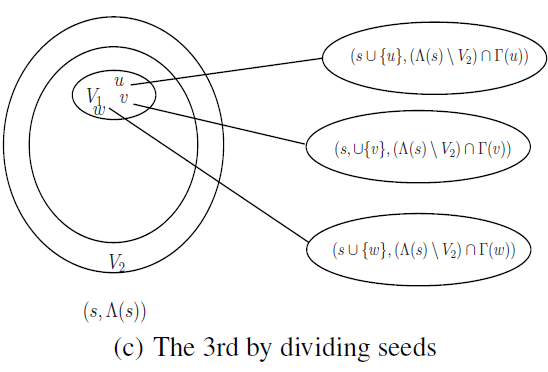
\includegraphics[scale=.8]{img/imagen8.png}
\caption{Reducción dividiendo}
\label{Comandos}
\end{figure}
\\
\subsection{Búsqueda de arboles}
Discutimos las principales diferencias entre los enfoques existentes de ramificación y unión y nuestro nuevo enfoque en términos de árboles de búsqueda, para encontrar las camarillas máximas en gráficos masivos. Deje que Td y Tb denoten el árbol de búsqueda por la marca existente y enfoques vinculados y los nuestros, respectivamente. Usamos nodo en lugar de vértice cuando hablamos de árboles. En Td, un nodo representa un par (C; P), donde C es una camarilla en crecimiento y P es su conjunto candidato. En Tb, un nodo representa una semilla (s; \begin{math}\Delta\end{math} (s)), donde la raíz de ambos árboles es (0; G). Un nodo en ambos árboles representa la misma información, porque s es un clique y \begin{math}\Delta\end{math} (s) es su conjunto candidato. Deje que un nodo hijo de (C; P) sea (C0; P0) en Td, y que un nodo hijo de (s; \begin{math}\Delta\end{math} (s)) sea (s0; \begin{math}\Delta\end{math} (s0)) en Tb. En Td, C0 = C U {u} donde u se selecciona de P, y P0 = \begin{math}\Delta\end{math} (C) n T(u) Los enfoques existentes de ramificación y unión conducen DFS sobre Td. En Tb, s0 = s [s0 y \begin{math}\Delta\end{math} (s0) = \begin{math}\Delta\end{math} (s) \ \begin{math}\Delta\end{math} (s0), donde s0 \begin{math}\Delta\end{math} (s). Realizamos BFS sobre Tb. Mostramos las diferencias entre Td y Tb. Vale la pena señalar que en Tb intenta seleccionar más vértices de \begin{math}\Delta\end{math} (s) para agrandar una camarilla en crecimiento en un nodo cuando se ramifica a su nodo hijo, mientras que en Td lo hace seleccionando un solo vértice v de P. En otras palabras, un borde en Tb representa una ruta en Td. Además, los vértices en X en Td pueden podarse mediante nuestro enfoque en Tb en una etapa temprana. Todo se debe a que los candidatos poco prometedores en \begin{math}\Delta\end{math} (s) serán podados lo antes posible. Inicialmente, la s de cualquiera (s, \begin{math}\Delta\end{math} (s)) en el conjunto inicial de semillas S es un triángulo abierto basado en el cual se da el límite inferior wc, y el límite superior ¡wc es maxcore + 1, y wt = |( ~wc + wc) /2|. En cada iteración de la búsqueda binaria, actualiza wc y ~wc al explorar el conjunto de semillas actual S. 
Primero: wc se mueve hacia abajo donde existe al menos una camarilla wc, lo que implica w(G) ≥ wc. 
Segundo: ~wc se mueve hacia arriba donde no hay cliques (~wc + 1), lo que implica w(G) ≤ ~wc.
Tercero: wT indica que es posible encontrar wT-camarillas entre wc y ~wc. Al encontrar a wT-clique, podemos movernos wc a wT, y al encontrar todas las semillas vacías en wt, podemos mover ~wc a wt - 1. 
\\
\begin{figure}[h!]
\centering
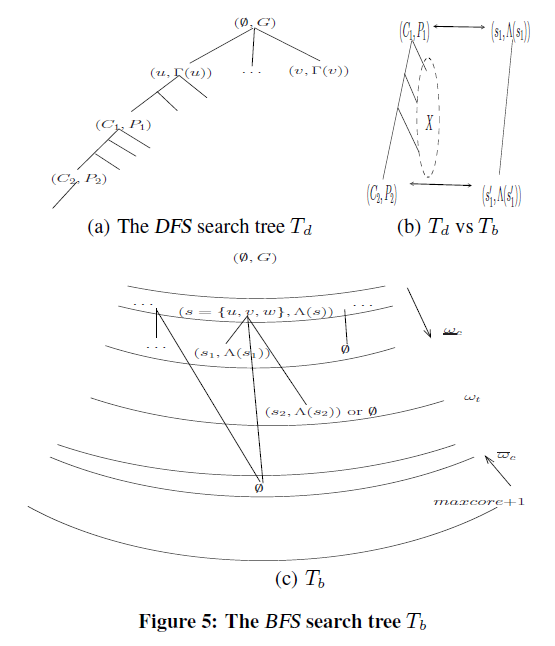
\includegraphics[scale=1]{img/imagen9.png}
\caption{Dividing Seeds}
\label{Comandos}
\end{figure}
\\
\subsection{El nuevo enfoque RMC} 
\\
\begin{figure}[h!]
\centering
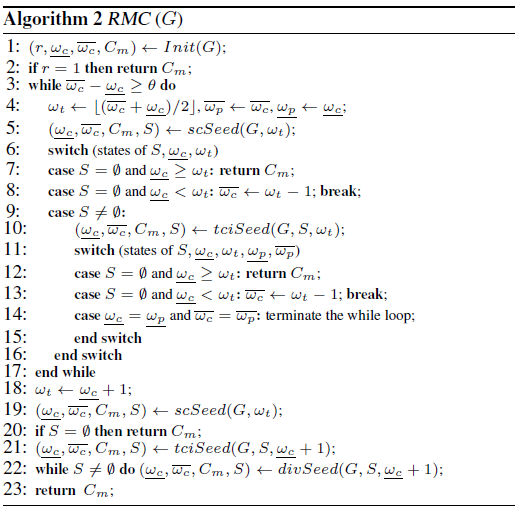
\includegraphics[scale=.8]{img/imagen10.png}
\caption{RMC}
\label{Comandos}
\end{figure}

\begin{figure}[h!]
\centering
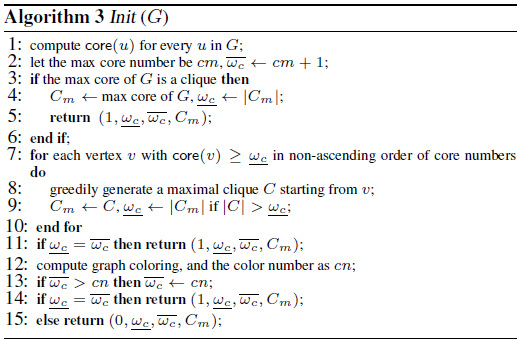
\includegraphics[scale=1]{img/imagen11.png}
\caption{Init}
\label{Comandos}
\end{figure}
Le damos nuestro algoritmo RMC ((Randomized Maximum Clique) en Algorithm 2. En Algorithm 2, el algoritmo Init (Algorithm 3) inicializa wc, ~wc, y Cm, y devuelve una variable r indica si la camarilla máxima ya se encuentra en el gráfico G (Línea 1). Si r = 1, entonces Cm es la camarilla máxima, el algoritmo termina devolviendo Cm (Línea 2). De lo contrario, aplica una búsqueda binaria para reducir la brecha entre el límite inferior wc y el superior enlazado ~wc en un ciclo while (Línea 3-17). El ciclo continuará si la diferencia entre wc y ~wc es mayor o igual que un umbral. En otras palabras, la búsqueda binaria se detendrá si otras iteraciones no reducen significativamente el espacio de búsqueda. En cada iteración, intentamos encontrar a wT-clique, donde b (wc + ~wc) = 2c (Línea 4). Primero, usamos un algoritmo aleatorio scSeed (Algoritmo 4) para actualizar wc y ~wc, y obtenemos un conjunto de semillas S donde posiblemente existen t-cliques (Línea 5). Aquí, scSeed aplica un muestreo uniforme en los bordes de G para extraer semillas si = (u; v; w) st (u; v) y (u; w) se muestrean y (v; w) es un borde en G. Vale la pena señalar que una semilla es un triángulo abierto. Como lo demuestra el Teorema 7.1, con alguna probabilidad de muestreo específica p, cada camarilla contiene al menos una semilla con alta probabilidad. Para cada semilla si, scSeed aplica la descomposición del núcleo [5] en \begin{math}\Delta\end{math} (si), poda los vértices que existen en no wT-cliques, y mueve vértices que se conectan a todos los demás a si. Esto da como resultado un límite superior ~wI y un límite inferior wI de w(Si [\begin{math}\Delta\end{math} (si)). Utilizamos los límites obtenidos para las semillas juntos para actualizar wc y ~wc, que a cambio elimina las semillas sin fruto y hace que S sea mínimo.
\subsection{Inicialización - Algorithm Init (Algorithm 3)}

Toma un gráfico G como entrada y devuelve una tupla de 4. Aquí, Cm es una clique, wc y ~wc son los límites inferior y superior, y r es un indicador de si Cm es la camarilla máxima.
Primero calculamos el número de núcleo para cada vértice u en G, denotado como núcleo (u), utilizando el algoritmo de descomposición del núcleo (línea 1). El número de núcleo máximo sea cm e inicialice wc como cm + 1. Si el núcleo máximo se encuentra como una camarilla, entonces se encuentra la camarilla máxima, devolviendo el resultado (línea 3-6). Discutimos cuándo el núcleo máximo de G no es una camarilla (Línea 7-15). Encontramos la camarilla Cm entre todas las camarillas máximas encontradas con avidez para cada vértice v si su número central (núcleo (v)) es el límite superior actual ~wc (Línea 7-10). Si los límites superior e inferior actuales son iguales, devolvemos el resultado ya que Cm encontrado es la camarilla máxima (Línea 11). A continuación, actualizamos aún más el límite superior actual usando el color del gráfico. Deje que el número central de G sea cn (Línea 12). ! c se reduce a cn si! c> cn. Finalmente devolvemos el resultado. Tenga en cuenta que en esta etapa, Cm encontrado es la camarilla máxima si wc = ~wc.
\\
\subsection{El muestreo y la reducción del núcleo - algoritmo scSeed (Algoritmo 4)}
La segunda fase es actualizar S usando la reducción por k-core (Ec. (1)). Ampliamos sy reducimos \begin{math}\Delta\end{math} (s) para cada semilla (s; \begin{math}\Delta\end{math} (s)) en S, y eliminaremos todo (s; \begin{math}\Delta\end{math} (s)) de S si no puede ayudar a encontrar una k-camarilla donde k se proporciona como una entrada del algoritmo (línea 7-33).
En la primera fase, muestreamos un conjunto de bordes del conjunto de bordes E de G, denotado como Es, usando un muestreo uniforme. Luego construimos el conjunto inicial de semillas S. Para cada semilla, (s; \begin{math}\Delta\end{math} (s)), en S, s es un triple abierto s = (u; v; w) si ambos (u; v) y (u; w) están en el conjunto de bordes muestreados Es y (v; w) están en E. Para cada semilla (s; \begin{math}\Delta\end{math} (s)), determinamos su límite superior! s como minfcore (u); núcleo (v); núcleo (w) g +1. Discutimos la probabilidad de muestreo p.
\\
\textbf{Teorema 7.1:} Sea Es un subconjunto de E de G mediante un muestreo uniforme de bordes de G con una probabilidad de muestreo de bordes p. Sea ST un conjunto de triángulos abiertos, s = (u, v, w), de modo que tanto (u, v) como (u, w) estén en Es y (v; w) estén en E. Cada k-camarilla en G contiene al menos un triángulo en ST con probabilidad \begin{math} 1 – n^(c)\end{math}, donde n es el número de vértices en G.
\\
\begin{figure}[h!]
\centering
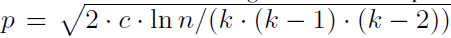
\includegraphics[scale=.8]{img/imagen12.png}
\label{Comandos}
\end{figure}
\\
\textbf{Bosquejo de prueba}
\\
Supongamos que E1 denota el evento de que uno de esos triángulos abiertos específicos se muestrea a partir de G. Luego, deje que E denote el evento de que se muestree al menos un triángulo abierto para una camarilla k, y deje que E denote que el evento E no ocurre.
\\
\begin{figure}[h!]
\centering
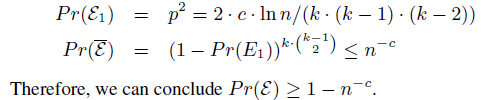
\includegraphics[scale=.8]{img/imagen13.png}
\label{Comandos}
\end{figure}
\\
\textbf{En la segunda fase}, actualizamos cada semilla (s; \begin{math}\Delta\end{math} (s)) en S y actualizamos S siguiendo el orden no ascendente en los límites inferiores (wS). Es importante tener en cuenta que la k inicial en el bucle (línea 7-33) es la entrada k del algoritmo para una k-clique y k puede aumentar para podar más semillas de S.
Primero, si ws de una semilla (s, \begin{math}\Delta\end{math} (s)) es menor que k, la semilla se eliminará de S, ya que no puede conducir a una k-camarilla (Línea 8) En segundo lugar, verificamos si se puede encontrar una k-camarilla en (s, \begin{math}\Delta\end{math} (s)) por la condición de |\begin{math}\Delta\end{math} (s) | + |s| <k. Si esta condición no se cumple, la semilla se eliminará de S (Línea 9-11). 
\\
En tercer lugar, actualizamos más una semilla si la condición no se cumple (Línea 12-31). Discutimos el tercer caso a continuación. Supongamos que encontramos que \begin{math}\Delta\end{math} (s) forma una camarilla, actualizamos la camarilla máxima actual Cm por (s; \begin{math}\Delta\end{math} (s)) y actualizamos el límite inferior actual para que sea wc = |Cm|. Vale la pena señalar que en cada iteración k permanece sin cambios o aumenta. Por lo tanto, el Cm actualizado no puede ser más pequeño que el encontrado anteriormente. Eliminamos (s, \begin{math}\Delta\end{math} (s)) de S, ya que es la camarilla máxima actual. Seguimos la ecuación. (1), calcular Xk, elimine Xk de \begin{math}\Delta\end{math} (s) y calcule F (línea 16-18). Aquí, Xk es un subconjunto de vértices en \begin{math}\Delta\end{math} (s) donde cada vértice u tiene un número central que es menor que k - |s| -1. F es un subconjunto de vértices en \begin{math}\Delta\end{math} (s) n Xk donde cada vértice se conecta a todos los demás vértices en \begin{math}\Delta\end{math} (s) n Xk. En otras palabras, s U F posiblemente puede formar una camarilla máxima. Hay varios casos:
\\
Caso-i) Cuando \begin{math}\Delta\end{math} (s) n F =0: Si (s, \begin{math}\Delta\end{math} (s)) no puede conducir a una k-clique porque F está vacío, la semilla (s, \begin{math}\Delta\end{math} (s)) se eliminará de S (Línea 19-21). De lo contrario, si F no está vacío, la camarilla máxima actual Cm puede actualizarse con s U F, y la semilla puede eliminarse de S, ya que la semilla se trata como la camarilla máxima actual (Línea 21-23).
\\
Caso-ii) cuando \begin{math}\Delta\end{math} (s) n F 6 =0: aumentará s por s [F y reducirá \begin{math}\Delta\end{math} (s) por \begin{math}\Delta\end{math} (s) n F. Además, si js [Fj + 1 k, implica se ha encontrado una k-clique (Línea 24), y actualizaremos el actual
camarilla máxima por un subgrafo con s [F [fvg donde v se toma de \begin{math}\Delta\end{math} (s) n F (Línea 25). Tenga en cuenta que el límite inferior wc se actualiza cuando se actualiza la camarilla máxima actual. Después de considerar los casos, actualizamos k para que sea wc +1 if wc ≥ k (Línea 31). Finalmente, devolvemos (wc, ~wc; Cm; S) donde ~wc es el número de núcleo del núcleo máximo encontrado para semillas no vacías.
\\
\begin{figure}[h!]
\centering
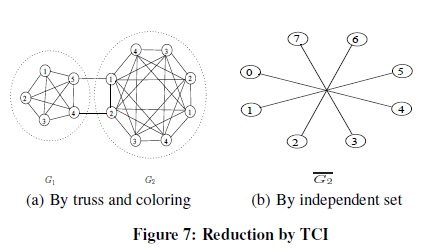
\includegraphics[scale=1]{img/imagen14.png}
\caption{Dividing Seeds}
\label{Comandos}
\end{figure}
\\
\subsection{La reducción por TCI}
El algoritmo tciSeed se muestra en el Algoritmo 5, que toma 3 entradas, un gráfico G, un conjunto de semillas S y un valor específico de k-clique k, y devuelve una tupla de 4 (wc, ~wc, Cm, S), donde wc y ~wc son un límite inferior y un límite superior, y Cm es la camarilla máxima actual, y S es un conjunto de semillas reducido. Como se da en la ecuación. (2), en tciSeed, para cada semilla (s, \begin{math}\Delta\end{math} (s)) / S, reducimos \begin{math}\Delta\end{math} (s) para que sea \begin{math}\Delta\end{math} (s) n (Xt U Xc), donde Xt y Xc son dos subconjuntos en \begin{math}\Delta\end{math} (s) de manera que cualquier vértice en Xt U Xc no pueda aparecer en una k-camarilla. Aquí Xt contiene los vértices que no pueden estar en un (wT-|s|) -truss en \begin{math}\Delta\end{math} (s), y Xc contiene vértices cuyos vecinos están coloreados con menos de wt - |s| - 1 colores La corrección de Xt es obvia.
\\
\textbf{Teorema 7.2:} Dado un gráfico G con un color gráfico, si w(G) ≥ k, entonces cualquier vértice v con vecinos coloreados con menos de k - 1 colores no se pueden incluir en ninguna k-camarilla de G.
Bosquejo de prueba: Suponga lo contrario, es decir, hay un vértice v cuyos vecinos se pueden colorear con menos de k - 1 colores, mientras que v se incluye en una k-camarilla. Entonces, el subgrafo inducido por {v} U T(v) contiene una k-camarilla y se puede colorear con menos de k colores, lo que conduce a una contradicción. Por lo que agrandamos s en la semilla de (s, \begin{math}\Delta\end{math} (s)) por un subconjunto P \begin{math}\Delta\end{math} (s), donde todos los vértices en P pertenecen a una camarilla máxima en \begin{math}\Delta\end{math} (s). Encontramos P como los vértices en un conjunto independiente máximo en el gráfico complementario ~\begin{math}\Delta\end{math}(s) en un algoritmo compIS, basado en el teorema 7.3.
\\
\textbf{Teorema 7.3:} En un gráfico G, si hay un vértice v con grado (v) = 1, hay al menos un conjunto independiente máximo de G que contiene v en G.
\\
\textbf{Bosquejo de prueba:} Suponga lo contrario, es decir, ninguno de los conjuntos independientes máximos contiene v en G. Suponga que I es un conjunto independiente máximo en G. Deje que el vecino único de v sea u. Solo hay dos casos relacionados con la existencia de u en I. Primero, si u € I, podemos tener un conjunto independiente máximo I0 reemplazando u con v de modo que I` -> I U {v} \ {u}. En segundo lugar, si u = €(no existe en) I, podemos tener un conjunto independiente más grande I0 ampliando I a I [fvg de modo que I` -> I U{v}.
Esto lleva a la conclusión de que al menos un conjunto independiente máximo contiene v.
\\
\begin{figure}[h!]
\centering
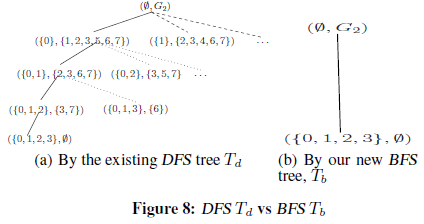
\includegraphics[scale=1]{img/imagen15.png}
\caption{DFS vs BFS}
\label{Comandos}
\end{figure}
\\
\textbf{La reducción dividiendo}
Hay casos en los que la búsqueda por fuerza bruta es inevitable, en tales casos son cuando S no está vacío. Mediante la búsqueda de fuerza bruta existente, para cada semilla (s; \begin{math}\Delta\end{math} (s)) en S, se ramifica desde cada vértice v \ \begin{math}\Delta\end{math} (s) para enumerar camarillas máximas y podar ramas sin fruto.
\\
\begin{figure}[h!]
\centering
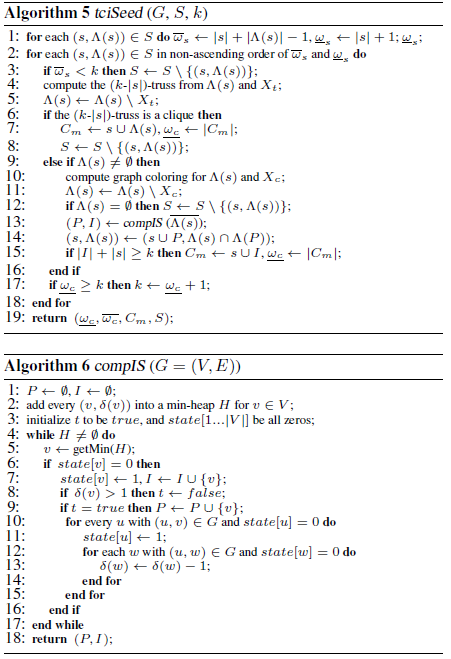
\includegraphics[scale=1]{img/imagen16.png}
\caption{Algoritmos}
\label{Comandos}
\end{figure}
\\
Como se indica en RMC (Algoritmo 2) en la Línea 22, encontramos la camarilla máxima del conjunto de semillas S llamando al algoritmo divSeed hasta que S se vacíe.
El Algoritmo divSeed se da en el Algoritmo 7, que toma 3 entradas: el gráfico G, el conjunto de semillas S y el valor ak para una k-camarilla específica. Tal valor k ofrece más oportunidades para que divSeed pueda podar. Al igual que scSeed y tciSeed, divSeed devuelve 4 tuplas (wc, ~wc, Cm, S). A diferencia de scSeed y tciSeed, divSeed devuelve un conjunto de semillas, denotado como S0, para reemplazar la entrada S. Aquí, una semilla (s, \begin{math}\Delta\end{math} (s)) \ S se reemplaza por varias semillas más pequeñas y densas (s0, \begin{math}\Delta\end{math} (s0)) en S0. Para cada semilla (s, \begin{math}\Delta\end{math} (s)) en S, calculamos V1 y V2. Como se discutió, V1 es un subconjunto de \begin{math}\Delta\end{math} (s) donde cada vértice en V1 tiene un color mayor o igual a k - |s|, y V2 es un subconjunto de \begin{math}\Delta\end{math} (s) donde por cada vértice en V2 sus vecinos en \begin{math}\Delta\end{math} (s) pueden colorearse con menos de k - |s| -1 colores (Línea 3-4). Según el teorema 7.2, los vértices en V2 no pueden estar en una k-camarilla. Eliminamos los vértices en V2 de \begin{math}\Delta\end{math} (s), y refinamos V1 para que sea V1 n V2 (Línea 5). Mostramos que cualquier k-clique de s [\begin{math}\Delta\end{math} (s) debe contener al menos un vértice de un subconjunto V1 \begin{math}\Delta\end{math} (s) Teorema 7.4.
\\
\textbf{Teorema 7.4:} Para un gráfico G, si w(G) k, entonces cualquier k-clique de G debe contener al menos un vértice con el color k.
\\
\textbf{Bosquejo de prueba:} Mostramos la afirmación por contradicción, es decir, suponemos que hay una camarilla k con todos los vértices coloreados <k en G. Luego, la coloración sigue siendo válida si eliminamos todos los otros vértices que no están incluidos en la camarilla k. Esto implica que obtenemos un color para una camarilla k que usa <k colores, lo que lleva a una contradicción. Por lo tanto, cualquier k-clique en G contiene al menos un vértice con color k. 2
\\
En divSeed, en el bucle (Línea 6-28), obtenemos una nueva semilla más pequeña / más densa, (s0, \begin{math}\Delta\end{math} (s0)) de la semilla actual (s, \begin{math}\Delta\end{math} (s)) para cada vértice v en V1. Aquí, s0 se convierte en s U {v}, y \begin{math}\Delta\end{math} (s0) se convierte en \begin{math}\Delta\end{math} (s) \T(v) (Línea 7). Luego, reducimos la nueva semilla (s0; \begin{math}\Delta\end{math} (s0) usando técnicas similares utilizadas en el algoritmo tciSeed (línea 6-28).
\\
\begin{figure}[h!]
\centering
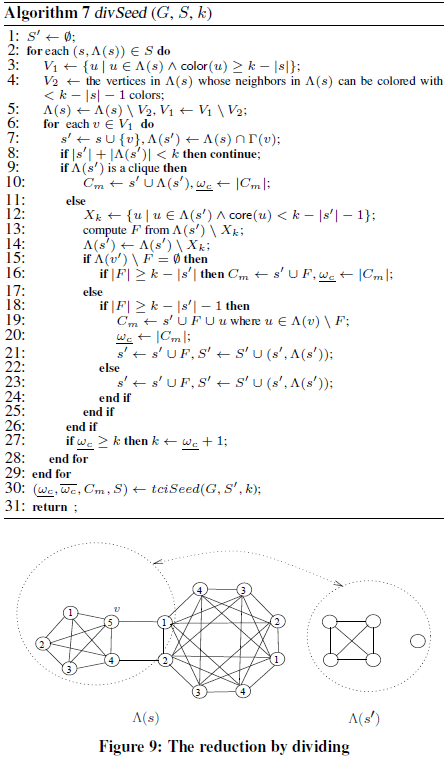
\includegraphics[scale=.9]{img/imagen17.png}
\caption{Algoritmo divSeed}
\label{Comandos}
\end{figure}
\\
\section{Estudios experimentales}
Hemos realizado estudios experimentales utilizando 22 gráficos grandes reales para comparar RMC con varios enfoques de vanguardia, incluyendo FMC, PMC, MCQD, cliquer, que son algoritmos exactos y GRASP [1], que es un algoritmo de aproximación en una maquina con CPU Intel Core i7-4770 de 3.40 GHz, 32 GB de RAM y Linux. La unidad de tiempo utilizada es la segunda y establecemos el límite de tiempo en 24 horas.
Delicious, Digg, Flixster, Foursquare, Friendster y Lastfm se descargan de http://socialcomputing.asu.edu/pages/conjuntos de datos La información detallada de los conjuntos de datos del mundo real se resume en la Tabla 1.
\\
\begin{figure}[h!]
\centering
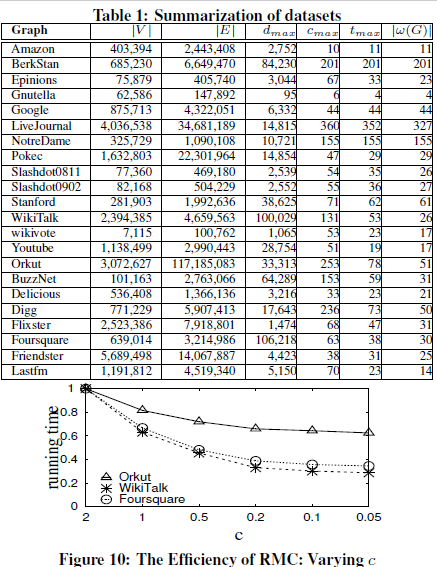
\includegraphics[scale=1]{img/imagen18.png}
\caption{Dataset}
\label{Comandos}
\end{figure}
\\
\textbf{La eficiencia en conjuntos de datos reales: La Tabla 2} muestra la eficiencia de RMC y sus comparaciones. Las columnas 12 y 15 muestran los tamaños de las camarillas máximas encontradas por GRASP y RMC, respectivamente. Descuidamos los resultados de otros algoritmos ya que son algoritmos exactos.
Como se demostró, RMC supera a todos los demás en todos los conjuntos de datos probados significativamente. De la Tabla 2, RMC, PMC y FMC superan significativamente a MCQD, cliquer y GRASP en la mayoría de los gráficos.
\\
\begin{figure}[h!]
\centering
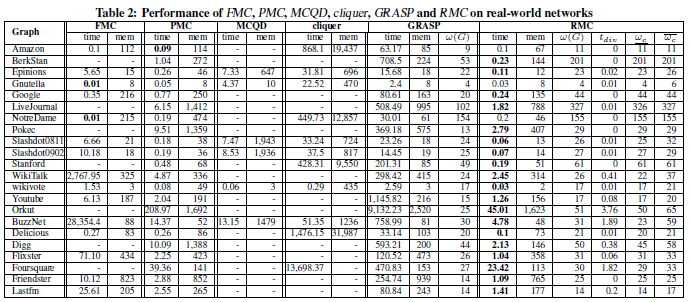
\includegraphics[scale=.85]{img/imagen19.png}
\caption{Performance}
\label{Comandos}
\end{figure}
\\
\textbf{La influencia del parámetro c:} Mostramos la influencia de c en el Teorema 7.1 en la precisión y eficiencia de RMC. Aquí mostramos los resultados utilizando 3 conjuntos de datos: Orkut, WikiTalk y Foursquare. Los conjuntos de datos restantes son similares a uno de los tres. La Fig. 10 demuestra el tiempo de ejecución empleando diferentes valores de c. Aquí, establecemos el tiempo de ejecución como 1 cuando c = 2, y usamos la relación para indicar el tiempo de ejecución con c menor. Como puede verse
\\
\begin{enumerate}
    \item Emplear c más pequeño mejora significativamente el rendimiento de RMC,
    \item La mejora es marginal cuando c es lo suficientemente pequeña, y
    \item La mejora difiere significativamente en diferentes gráficos.
    \item La influencia de c en la precisión de RMC se muestra en la Tabla 3.
\end{enumerate}
\\
\begin{figure}[h!]
\centering
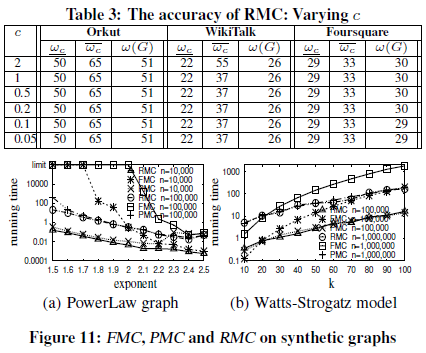
\includegraphics[scale=1]{img/imagen20.png}
\caption{Table 3}
\label{Comandos}
\end{figure}
\\
\section{Conclusión}
Nuestro enfoque RMC emplea un esquema de búsqueda binaria. Específicamente, RMC mantiene un límite inferior wc y un límite superior ~wc de w(G) e intenta encontrar una wT-clique en cada iteración donde wT = b (wc +~wc) = 2c. Debido a lo incompleto de NP de encontrar un wT-clique en cada iteración, RMC muestrea un conjunto de semillas S st encontrar a! T-clique en el gráfico G es equivalente a encontrar una wT-clique en S con garantías de probabilidad \begin{math}(1 – n^(-C)) \end{math}. Para las semillas restantes cuyas camarillas máximas probablemente puedan actualizar la camarilla máxima Cm encontrada hasta ahora, proponemos un nuevo algoritmo iterativo de búsqueda de fuerza bruta divSeed para encontrar la camarilla máxima cuando el conjunto de semillas S se vacía.

\chapter{Lenguaje y Paquetes}
\section{Lenguaje}
El lenguaje que se utilizó fue Java, ya qué es un lenguaje con el cual todos los integrantes están familiarizados y tienen experiencia. De igual manera es un lenguaje amigable para aplicaciones GUI e interfaces, lo cual nos ayudó mucho para el dibujo de grafos.

\section{Paquetes utilizados}
java.awt.event.ActionEvent: Un evento semántico que indica que ocurrió una acción definida por componentes. Este evento de alto nivel es generado por un componente (como lo son los  botones en nuestro programa) cuando ocurre la acción específica del componente (como ser presionado). El evento se pasa a todos los objetos ActionListener​ ​ que se registraron para recibir dichos eventos utilizando el método addActionListener​ ​ del componente 
\\\\
import java.util.*;  
\\\\
import java.util.ArrayList:  La usamos para los objetos ArrayList y usarlos en una lista redimensionable en la que tendremos disponibles los métodos más habituales para operar con listas. Los usamos para extraer, construir e imprimir los elementos grafos y aristas. 
\\\\
import javax.swing.JFileChooser: Es una forma rápida y fácil de solicitar al usuario que elija un archivo o una ubicación para guardar archivos. Lo usamos para subir imagenes de fondo para interpretar un mapa con los grafos. 
\\\\
import javax.swing.JOptionPane. 
\\\\ 
import java.awt.BasicStroke:  Analiza las subrutas no cerradas y segmentos de guión que se extienden más allá del final. Con sus métodos encontramos los nodos que encierran las aristas.  import java.awt.Color: Lo usamos para cambiar los colores de los objetos en la interfaz. 
\\\\
import java.awt.Graphics: Lo usamos para las operaciones graficas. 
\\\\ 
import java.awt.Graphics2D: Amplía la clase Graphics, haciendo uso de sus métodos podemos darle valores enteros a los nodos, son los números que se ven junto a los nodos. 
\\\\ 
import java.awt.RenderingHints. 
       
\chapter{Uso de la aplicación}
\section{Pantalla principal}

\begin{figure}[h!]
\centering
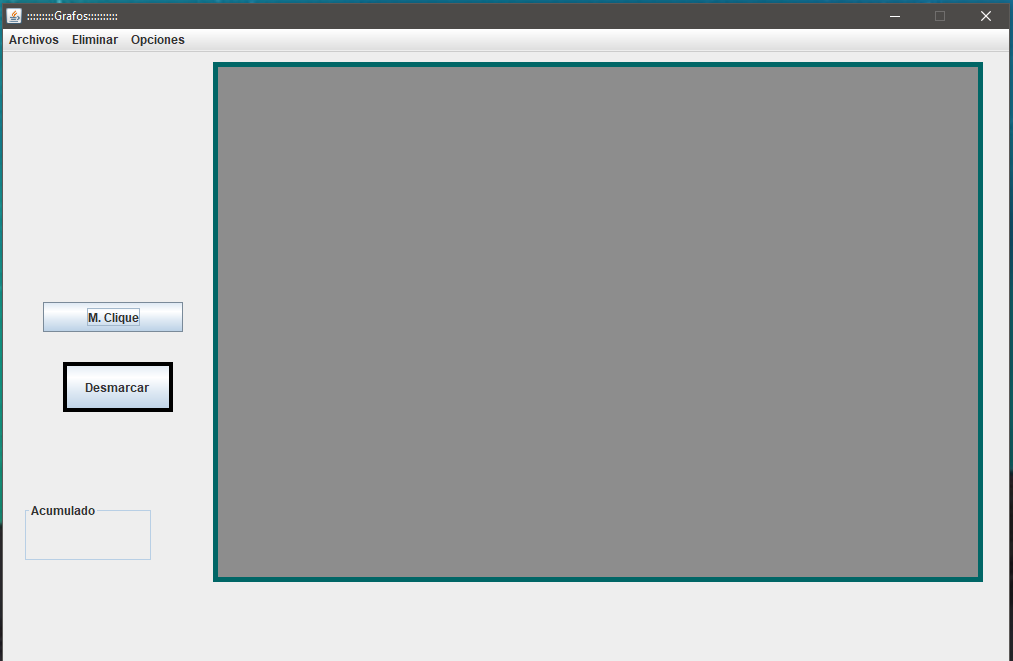
\includegraphics[scale=.6]{img/principal.png}
\caption{Pantalla principal}
\label{Comandos}
\end{figure}
\\
Al comenzar la aplicación se puede observar una pantalla en la cual se tiene en un principio un fondo gris, el cual usaremos para dibujar nuestros grafos. 
\\
Del lado izquierdo tenemos un botón para calcular el máximo cliqué y un botón de Desmarcar que de momento no tiene función. En la parte superior se tiene una serie de opciones que nos ayudarán en diversas situaciones; las cuales veremos más adelante con detalle.

\section{Dibujar un Grafo}
\subsection{Pintar Nodo}
Para dibujar un grafo solo se requiere dar click sobre la superficie gris que se aprecia al iniciar la aplicación. 
En donde se de click es donde se pintará el nodo de nuestro Grafo, entonces podemos comenzar a dibujar los nodos que compongan nuestro grafo. 

\begin{figure}[h!]
\centering
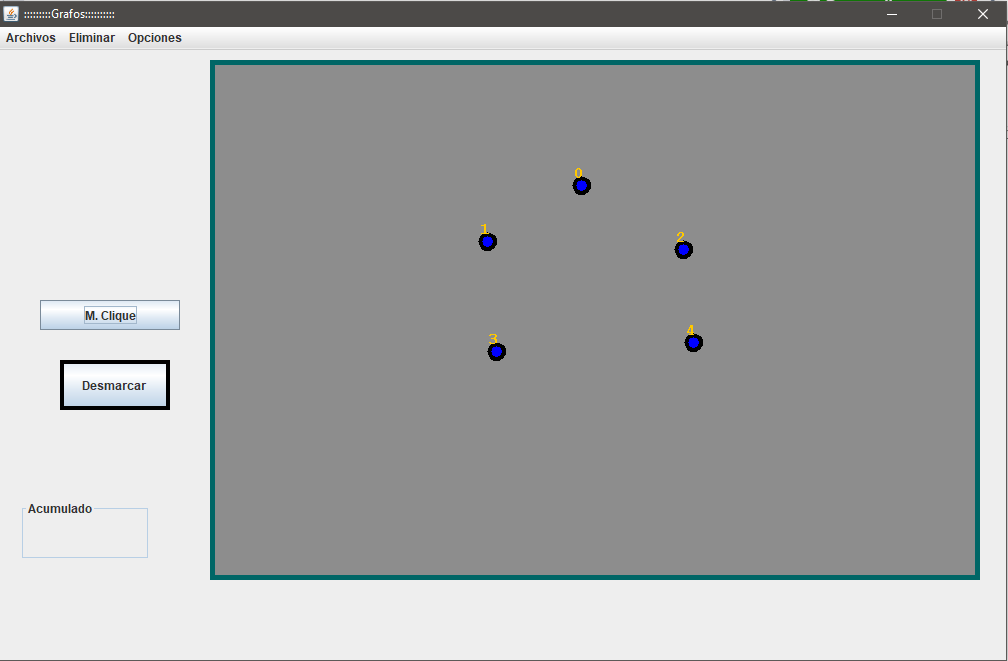
\includegraphics[scale=.5]{img/grafo.PNG}
\caption{Dibujar nodos}
\label{Comandos}
\end{figure}

\subsection{Unir Nodos}
Para unir los nodos de nuestro Grafo lo primero que haremos sera dar click en un nodo, el cuál será nuestro origen y luego dar click sobre el nodo destino para que exista una unión entre ellos. Al realizar esto nos abrirá una pequeña ventana donde tendreos que teclear el peso que habrá entre estos dos nodos, ya qué de igual forma el programa funciona para calcular el camino más corto.
\\
Realizar esto para unir todos los nodos que tengan relación en nuestro grafo.
\\
Al final tendremos pintado nustro grafo para poder caluclar el máximo cliqué o calcular el camino más corto. 

\begin{figure}[h!]
\centering
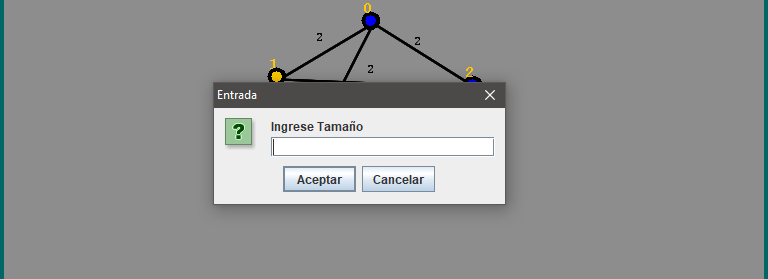
\includegraphics[scale=.35]{img/alert.PNG}
\caption{Definir peso de unión}
\label{Comandos}
\end{figure}

\begin{figure}[h!]
\centering
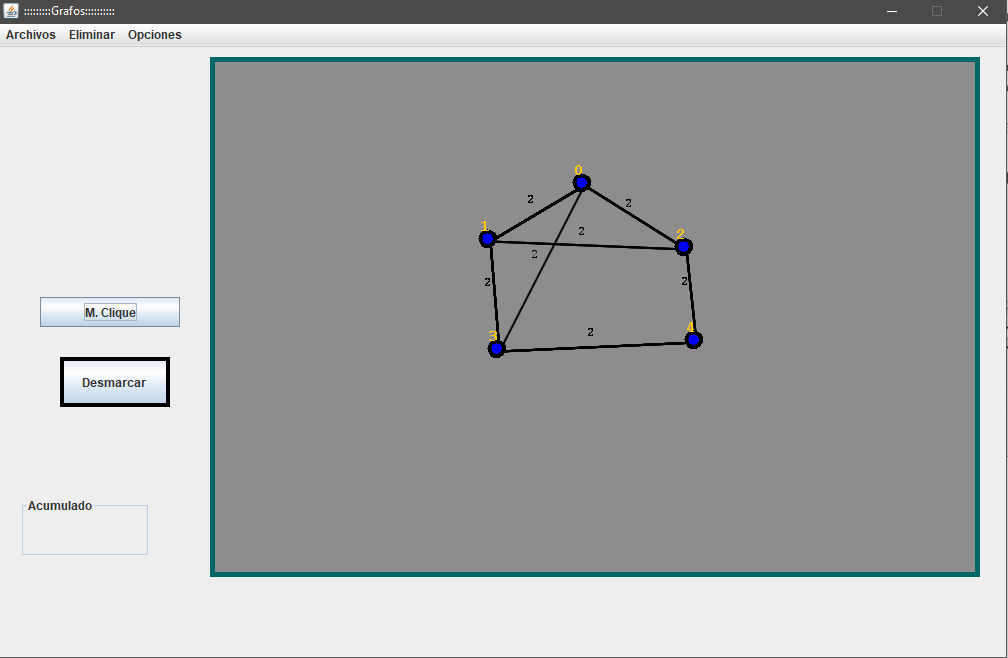
\includegraphics[scale=.5]{img/union.PNG}
\caption{Dibujar vertices}
\label{Comandos}
\end{figure}

\subsection{Utilizar muestra}
Si no se tiene un grafo para realizar alguna prueba se puede cargar un grafo que se encuentra a modo de muestra. 
\\
Nos dirigimos a la parte superior en la opcion de archivo damos click y nos desplazamos a la opción de Muestra. Al dar click en esta opción nos cargará un Grafo muestra con el cual podemos trabajar. 
\\
\begin{figure}[h!]
\centering
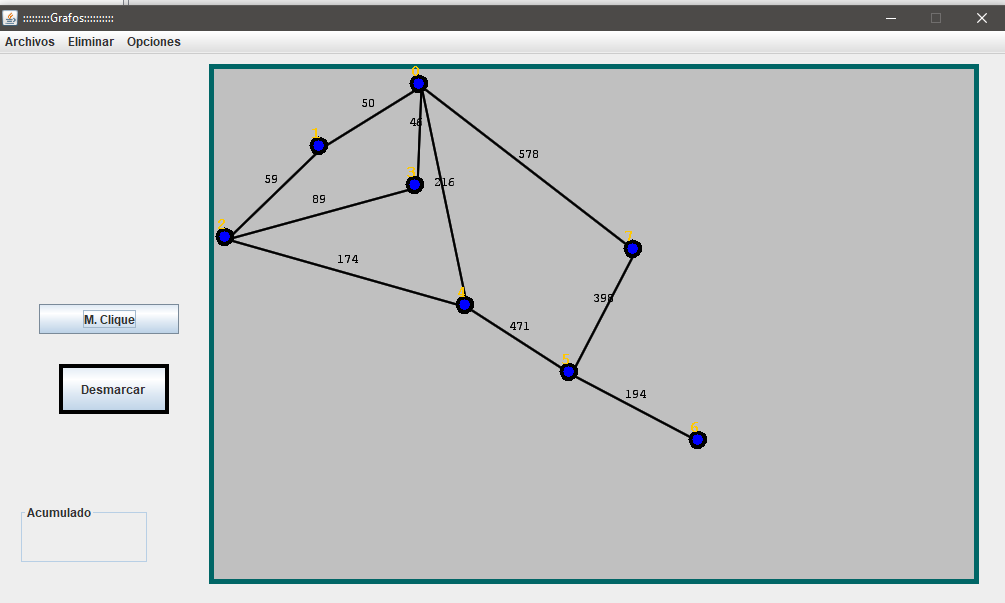
\includegraphics[scale=.45]{img/muestra.PNG}
\caption{Dibujar vertices}
\label{Comandos}
\end{figure}
\\
\section{Características}
\subsection{Eliminar Nodo}
Dentro de la aplicación es posible eliminar nodos si es que hubo algún error.\\
Para ello lo que se tiene que realizar es lo siguiente. 
 \begin{enumerate}
     \item Dirigirirnos a la parte superior donde dice Elimiar y dar click. 
     \item Se desplegará una lista de 3 opciones (Eliminar nodo, Eliminar Arista, Eliminar todas las aristas).
     \item Seleccionamos elimar Nodo, abrirá una pequeña ventana donde nos pedirá el nodo a eliminar.
     \item Digitamos el nodo y damos click en aceptar.
 \end{enumerate}
 \\
\begin{figure}[h!]
\centering
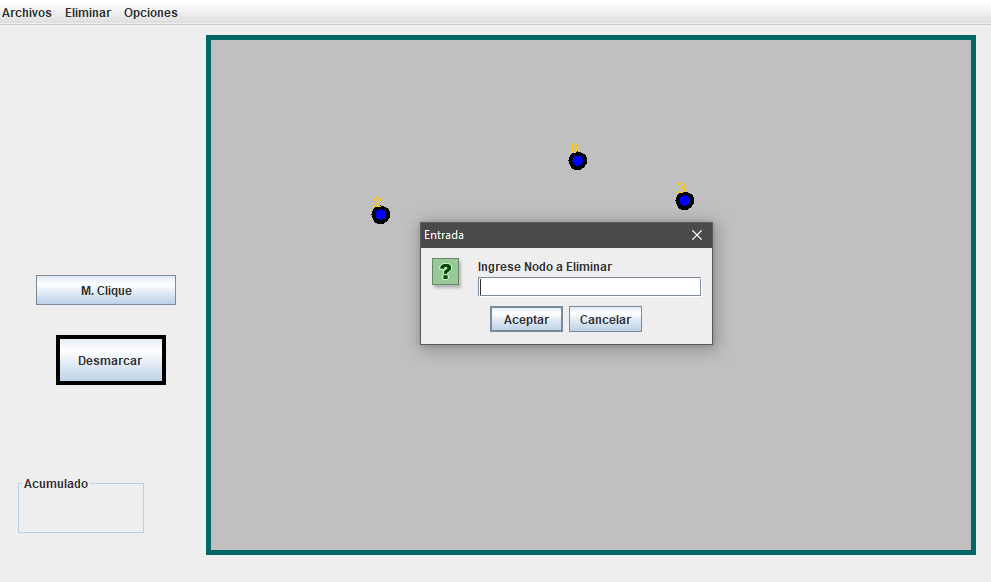
\includegraphics[scale=.55]{img/delete.PNG}
\caption{Eliminar Nodo}
\label{Comandos}
\end{figure}

\\
\subsection{Eliminar vertice o arista}
Para ello realizamos los mismos pasos que en eliminar nodo solo que seleccionamos la opción de eliminar arista, en esta ocación nos saldrá una ventana pero debemos digitar dos nodos para saber que arista eliminaremos.

\begin{figure}[h!]
\centering

\includegraphics[scale=1]{img/deleteA.PNG}
\caption{Eliminar vertice}
\label{Comandos}
\end{figure}

De igual manera podemos elimnar todos los vertices. Para esto solo se tiene que seguir los pasos antes mencionados para eliminar nodo y arista (vertice) pero ahora daremos click en Eliminar todas las aristas. 
\\
Al dar click se eliminarán todas las aristas existentes en nuestro grafo, esto nos ayuda a que si no tenemos muy claro en que estamos mal en el grafo poder empezar desde cero a realizar las relaciones.

\subsection{Cambiar color de fondo}
Es posible cambiar el color de fondo de nuestra área de trabajo. 
\\
Para ello solo tenemos que ir a la parte superior y dar click en la opción de opciones luego donde dice color, lo que nos abrirá del lado izquierdo una pequeña paleta de colores en donde el usuario podrá elegir entre 12 colores distintos, al dar click sobre cualquier color en automático se realizará el cambio de color de fondo para que se utilice al agrado de cada persona o dependiendo si es un lugar con mucha iluminacion, etc. 

\begin{figure}[h!]
\centering
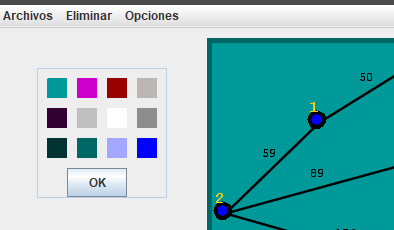
\includegraphics[scale=.75]{img/color.PNG}
\caption{Cambiar color}
\label{Comandos}
\end{figure}
\\
\subsection{Calcular Camino más corto}
Debido a que se tomó de un proyecto ya implementado el prgrama cuenta con la capacidad de calcular el camino más corto de un nodo a otro. 
\\
Si queremos utilizar esta caracteristica lo que necesitamos es seguir los pasos siguientes: 
\begin{enumerate}
    \item Dirigirnos a la parte superior y dar click en Archivos. 
    \item Seleccionar la opción de Camino más Corto. 
    \item abrirá una ventana para que indiquemos nodo origen y luego otra para el nodo destino. 
    \item Despues de ingresar los datos damos click y nos pintará de color la ruta del camino más corto.
\end{enumerate}
\\
\begin{figure}[h!]
\centering
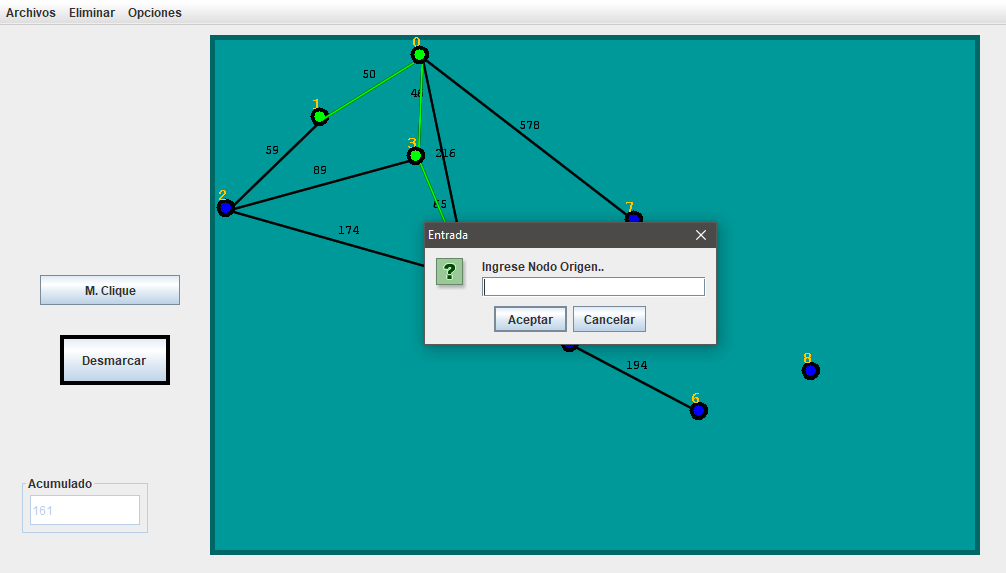
\includegraphics[scale=.6]{img/corto.PNG}
\caption{Cambiar color}
\label{Comandos}
\end{figure}
\\
\subsection{Cargar Mapas}
Una de las caracteristicaas y ventajas que pudimos econtrar e implementar en esta aplicación es el cargar cualquier mapa (imagen) de fondo para poder pintar el grafo sobre éste, de forma que se visualice un problema más real. Así, de igual manera sea amigable y entendible para el usuario. 
\\\\
Por ejemplo se puede cargar el mapa de algún Pais, mapa de alguna ruta de camiones, metro, suburbano, etc, para poder definir cual es la ruta más cerca para desplazarse de un punto a otro. 
\\
Podriamos cargar un mapa con imagenes de personas y definir gustos en común para determinar cual sería el mayor clique entre este grupo de personas. 
\\

\begin{figure}[h!]
\centering
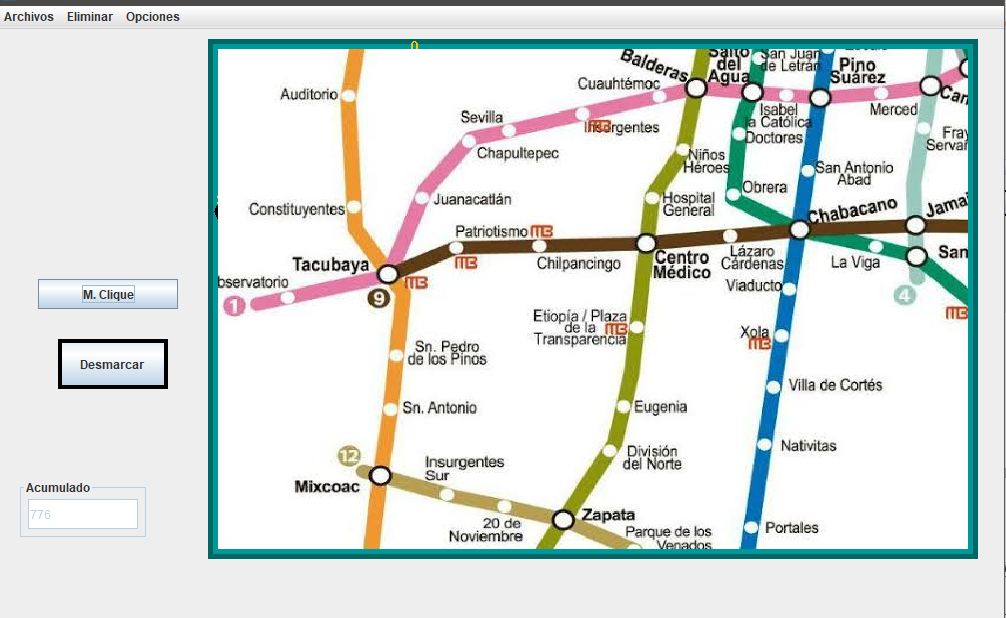
\includegraphics[scale=.6]{img/mapa.PNG}
\caption{Cambiar color}
\label{Comandos}
\end{figure}

\section{Calcular Máximo Cliqué}
Para poder calcular el Máximo Cliqué, tenemos que primero haber pintado un grafo con todo y sus relaciones entre nodos. 
\\
Ahora nos dirigimos al lado izquierdo de la pantalla donde se encuentra un botón que dice M.Clique y damos click. Al terminar el proceso del algoritmo se mostrará una pequeña ventana donde dice que se ha obtenido el máximo cliqué y el tamaño del mismo. Al cerrar la ventana podemos ver en la consola que nos imprime los nodos que conforman este máximo cliqué puede haber más de un máximo cliqué ya qué, puede que existan más de dos soluciones para el problema planteado.

\begin{figure}[h!]
\centering
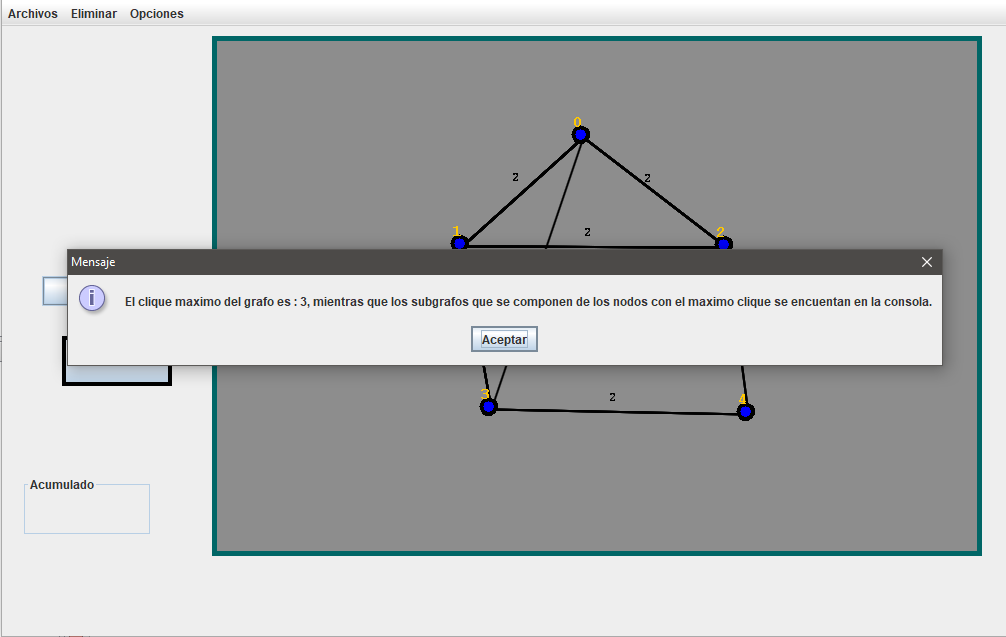
\includegraphics[scale=.58]{img/clique.PNG}
\caption{Calcular Máximo Cliqué}
\label{Comandos}
\end{figure}


\chapter{Conclusiones}

\section{Flores Aguilar Aldo Ignacio}
Como se mencionó antes, el equipo partió de un proyecto con el que ya contaba, el cual ya era capaz de visualizar un panel donde se podía dibujar grafos y mostrar el camino mínimo entre nodos. El equipo tuvo que emplear nuevas técnicas en java donde pudiera dar uso a métodos gráficos como eventos que pudieran ser usados como listas. Si se hubiera usado un método donde el usuario solo introdujera las matrices de adyacencia y de coeficientes; el programa hubiera sido mucho más simple de programar, pero el encanto de los grafos se encuentra en que estos tienen que ser gráficos, este tipo de esfuerzos se llevan a cabo para que el usuario pueda manejar el programa de una manera simple, y el equipo está de acuerdo en que el uso del proyecto es bastante intuitivo, me encuentro satisfecho con el funcionamiento del programa, pero espero poder desarrollarlo un poco más y resolver ciertas limitaciones que podrían presentarse.


\section{Mata Franco Carlos Jesus}
Finalmente con el termino del proyecto podemos encontrar que el problema del \textbf{Máximo Cliqué} tiene distintas aplicaciones en la vida real enfocadas principalmente en el análisis del comportamiento de ciertos individuos o elementos que tienen caracterisiticas o relaciones en común ya sea en el área social o en algún ámbito biologíco, etc. 
\\
En cuanto a la aplicación se pudo observar que cumple con el cálculo del máximo cliqué y que, se puede usar en un caso más real, ya qué como se mencionó antes se puede cargar un mapa o imagen para pintar el grafo sobre la misma. Además que es una interfáz amigable para el usuario tanto para el uso como para el entendimiento del resultado. 


\section{Ruiz González Ian Alexander}
Después de todo el trabajo realizado, encuentro la aplicación de algoritmos como algo más bastó de lo que pensaba. Tenía la idea de usar un algoritmo para cada cosa pero no me podía imaginar que un solo algoritmo tendría tantas aplicaciones diversas.
Partir de un problema similar al agente viajero y darle una perspectiva a grupos de redes sociales, adn, geología, solo para encontrar la mayor compatibilidad entre grupos de individuos, genes, etc. Es algo increíble!
El desarrollo del proyecto partiendo de que tenga una interfaz gráfica fue algo nuevo, no había tenido la necesidad de crearlas antes y descubrir algunos trucos en netbeans fue clave en todo esto, la simplicidad de nuestro programa lo hace útil para practicar en él y meterse de lleno al problema del clique máximo, el apartado de cargas mapas (aunque sólo sea una imagen) lo hace más útil a un aplicación real (Google maps en mini) y es mejor trabajar un ejercicio de este tipo con algo que puedas ver de forma práctica a solo con matrices o nodos.
       
          
         
         

        

